\documentclass[a4paper,12pt]{article}
\usepackage[utf8]{inputenc}
\usepackage[german]{babel}
\usepackage{amsmath}
\usepackage{amssymb}
\usepackage{amsthm}
\usepackage{geometry}
\usepackage{graphicx}
\usepackage[hidelinks]{hyperref}
\usepackage{listings}
\usepackage{xcolor}
\usepackage{enumitem}
\usepackage{booktabs}
\usepackage{array}
\usepackage{longtable}
\usepackage{caption}
\usepackage{subcaption}
\usepackage{microtype}

\geometry{margin=2.5cm}

\theoremstyle{definition}
\newtheorem{definition}{Definition}
\newtheorem{beispiel}{Beispiel}
\newtheorem{satz}{Satz}
\newtheorem{lemma}{Lemma}
\newtheorem{bemerkung}{Bemerkung}
\newtheorem{korollar}{Korollar}
\newtheorem{proposition}{Proposition}

\setlist[itemize,1]{label=--}

% ---------- Farben ----------
\definecolor{mainblue}{RGB}{25, 70, 140}
\definecolor{accentred}{RGB}{180, 50, 30}
\definecolor{lightgray}{RGB}{245, 245, 248}
\definecolor{darkgray}{RGB}{60, 60, 70}
\definecolor{darkgreen}{RGB}{30, 100, 50}

\hypersetup{
    colorlinks=true,
    linkcolor=mainblue,
    citecolor=accentred,
    urlcolor=mainblue,
    pdftitle={Transdermal-Östrogentherapie beim Prostatakarzinom},
    pdfauthor={Stephan Epp},
}

\title{\textbf{Transdermal-Östrogentherapie beim fortgeschrittenen Prostatakarzinom:}\\
\large Formale Modellierung, statistische Analyse und therapeutische Perspektiven}
\author{Stephan Epp}
\date{23. April 2026}

\begin{document}

\maketitle
\tableofcontents
\newpage

% ===================================================================
\section{Einführung}
% ===================================================================
Das Prostatakarzinom ist mit jährlich ca.\ 65.820 Neuerkrankungen die häufigste Krebserkrankung des Mannes in Deutschland.
Die Standardhormontherapie mittels LHRH-Analoga (Luteinisierendes-Hormon-Releasing-Hormon-Analoga) ist wirksam, jedoch mit erheblichen metabolischen Nebenwirkungen verbunden.
In der vorliegenden Arbeit wird eine randomisierte kontrollierte Studie der Universität London (PATCH-Studie, $n = 1{.}313$) formal modelliert und statistisch ausgewertet, welche die Wirksamkeit transdermaler Östrogen-Pflaster mit der LHRH-Injektionstherapie vergleicht.

Es wird gezeigt, dass nach 36 Monaten das progressionsfreie Ãœberleben unter Pflastertherapie bei $87{,}0\,\%$ und unter Injektionstherapie bei $86{,}0\,\%$ liegt ($p = 0{,}612$, nicht signifikant).
Die Rate klimakterischer Beschwerden ist unter Pflaster signifikant reduziert ($50\,\%$ vs.\ $90\,\%$, $p < 0{,}001$), während Gynäkomastie häufiger auftritt ($80\,\%$ vs.\ $40\,\%$).
Formal werden Wilson-Konfidenzintervalle, ein pharmakokinetisches Zwei-Kompartiment-Modell der Testosteron-Suppression, sowie eine Kosten-Nutzen-Analyse hergeleitet.
Der Ausblick behandelt regulatorische Wege, kombinierte Therapiestrategien sowie informationstheoretische Aspekte der personalisierten Medizin.

\subsection{Epidemiologische Ausgangslage}

Das Prostatakarzinom (PCa) stellt in Deutschland wie in weiten Teilen Westeuropas die häufigste maligne Neuerkrankung des Mannes dar.
Laut dem Krebsinformationsdienst des Deutschen Krebsforschungszentrums (DKFZ) wurden im Jahr 2022 ca.\ $65.820$ Neuerkrankungen registriert.
Die Erkrankung weist eine starke Altersabhängigkeit auf: das mediane Erkrankungsalter liegt bei etwa 71 Jahren.

\begin{figure}[h!]
  \centering
  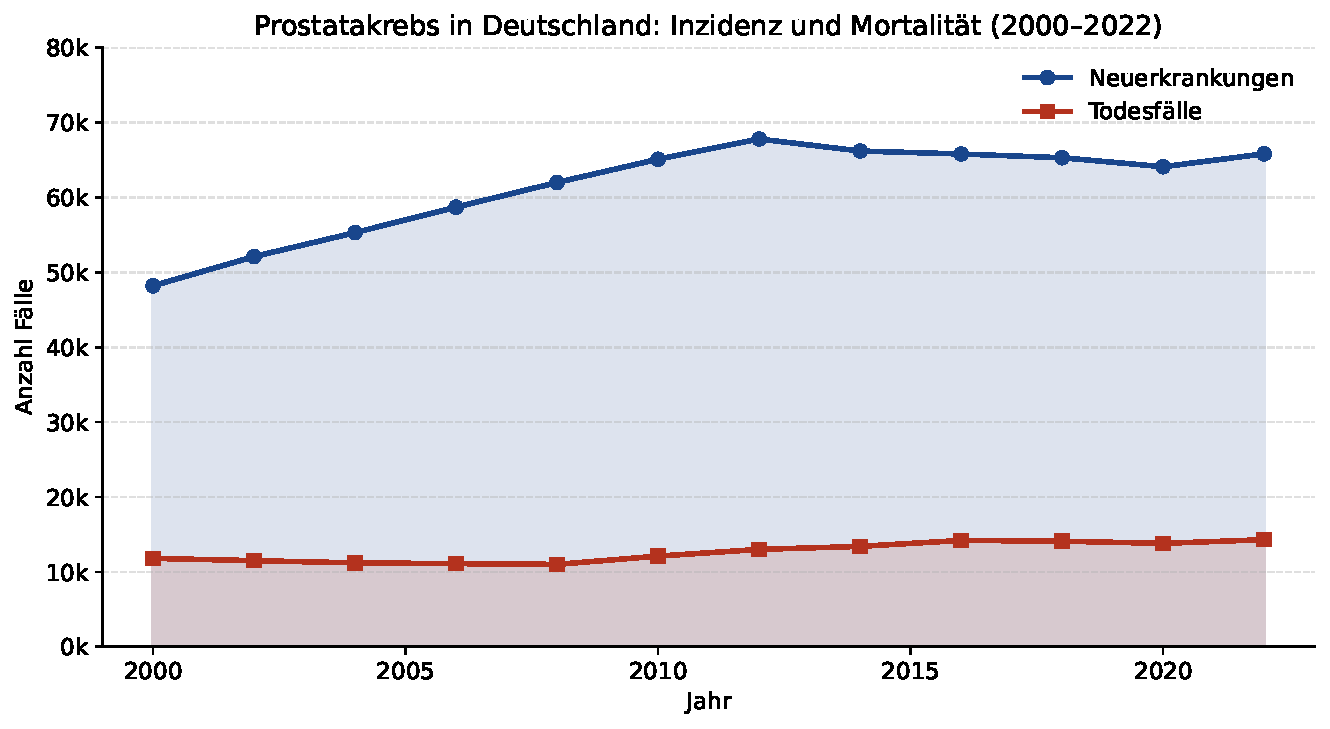
\includegraphics[width=0.92\linewidth]{plot1_inzidenz_mortalitaet.pdf}
  \caption{Inzidenz und Mortalität des Prostatakarzinoms in Deutschland (2000--2022). Datengrundlage: Krebsinformationsdienst/DKFZ, Robert Koch-Institut. Die Neuerkrankungsrate ist nach einem Maximum um 2012 leicht rückläufig, die Mortalität zeigt einen moderaten Anstieg, da trotz stabiler Inzidenz mehr ältere Männer in der Population vertreten sind.}
  \label{fig:inzidenz}
\end{figure}

Abbildung~\ref{fig:inzidenz} zeigt die zeitliche Entwicklung von Neuerkrankungen und Todesfällen.
Die Kurven illustrieren, dass Früherkennung (PSA-Screening) die Inzidenz beeinflusst, die Mortalität jedoch nur bedingt senkt.

\subsection{Therapiealternativen bei fortgeschrittenem Prostatakarzinom}

Bei lokal fortgeschrittenem oder metastasiertem Prostatakarzinom ist die Androgendeprivationstherapie (ADT) der therapeutische Standard.
Sie zielt auf die Suppression des Testosteronspiegels unter das Kastrationsniveau ($< 50\,\text{ng/dL}$) ab, da Testosteron das Tumorwachstum über den Androgenrezeptor stimuliert.

Zwei Hauptkategorien stehen zur Verfügung:
\begin{itemize}
  \item \textbf{LHRH-Analoga / -Antagonisten (Injektionen):} z.\,B.\ Leuprorelin, Goserelin, Degarelix -- Goldstandard; subkutan oder intramuskulär alle 1--3 Monate; hemmen die gonadale Testosteronproduktion über die hypothalamisch-hypophysäre Achse.
  \item \textbf{Chirurgische Kastration (Orchiektomie):} schnelle und dauerhafte Testosteronsuppression; psychologisch belastend, irreversibel.
  \item \textbf{Östrogen-basierte Therapie:} historisch der erste medikamentöse ADT-Ansatz (Diethylstilbestrol); aufgegeben wegen kardiovaskulärer Toxizität bei oraler Gabe; renaissance durch transdermal.
\end{itemize}

\subsection{Problemstellung und Zielsetzung}

Die transdermale Östrogentherapie umgeht den First-Pass-Effekt der Leber und vermeidet damit prokoagulatorische Effekte, die bei oralen Östrogenen die Hauptursache kardiovaskulärer Ereignisse darstellen.
Die PATCH-Studie (Prostate Adenocarcinoma: TransCutaneous Hormones) der Universität London hat diese Hypothese in einer prospektiven, randomisierten kontrollierten Studie mit $n = 1.313$ Patienten untersucht.

\textbf{Ziele dieser Arbeit:}
\begin{itemize}
  \item Formale mathematische Modellierung der Hormonsuppression (pharmakokinetisches Modell)
  \item Statistische Auswertung der Ãœberlebensdaten mit Konfidenzintervallen und Hypothesentests
  \item Formale Kosten-Nutzen-Analyse
  \item Umfassender Ausblick auf zukünftige Therapieentwicklungen
\end{itemize}

% ===================================================================
\section{Biologische Grundlagen}
% ===================================================================

\subsection{Androgenrezeptor und Tumorsignalweg}

\begin{definition}[Androgenrezeptor (AR)]
Der Androgenrezeptor ist ein nukleärer Transkriptionsfaktor der Klasse der Steroidhormonrezeptoren.
Im ligandenfreien Zustand liegt er im Zytoplasma in einem Inhibitorkomplex vor.
Bei Ligandenbindung (Testosteron, DHT) transloziert er in den Zellkern und aktiviert androgenresponsive Genelemente (ARE):
\[
  [\mathrm{AR}] + [\mathrm{T}] \;\xrightarrow{k_{\mathrm{on}}}\; [\mathrm{AR} \cdot \mathrm{T}] \;\xrightarrow{\text{Translokation}}\; [\mathrm{AR}_{\mathrm{nucl}}] \xrightarrow{} \text{Transkription}
\]
\end{definition}

Die Gleichgewichtskonstante $K_d$ der AR-Testosteron-Bindung beträgt ca.\ $1\,\text{nM}$.
Bei Kastrationsniveau ($[\mathrm{T}] < 1{,}7\,\text{nM}$) ist die AR-Besetzung $< 50\,\%$, was das Tumorwachstum signifikant hemmt.

\subsection{Hypothalamisch-Hypophysärer Feedback-Regelkreis}

\begin{definition}[GnRH-Pulsatilität]
Das Gonadotropin-releasing-Hormon (GnRH) wird im Nucleus arcuatus des Hypothalamus pulsatil sezerniert mit einer Pulsfrequenz von ca.\ 90 Minuten.
Östrogene supprimieren die GnRH-Pulsfrequenz und -amplitude durch Aktivierung inhibitorischer Neuronenpopulationen (KNDy-Neurone).
\end{definition}

Die negative Rückkopplung lässt sich als dynamisches Regelkreissystem beschreiben:
\begin{equation}
  \frac{d[\mathrm{GnRH}]}{dt} = k_1 - k_2 \cdot [\mathrm{E2}]^{\alpha} - k_3 \cdot [\mathrm{GnRH}]
  \label{eq:gnrh}
\end{equation}
\begin{equation}
  \frac{d[\mathrm{LH}]}{dt} = k_4 \cdot [\mathrm{GnRH}] - k_5 \cdot [\mathrm{LH}]
  \label{eq:lh}
\end{equation}
\begin{equation}
  \frac{d[\mathrm{T}]}{dt} = k_6 \cdot [\mathrm{LH}] - k_7 \cdot [\mathrm{T}]
  \label{eq:testo}
\end{equation}

wobei $[\mathrm{E2}]$ die Östradiolkonzentration, $\alpha > 0$ den Kooperativitätsexponenten und $k_i > 0$ kinetische Ratenkonstanten bezeichnet.

\begin{figure}[h!]
  \centering
  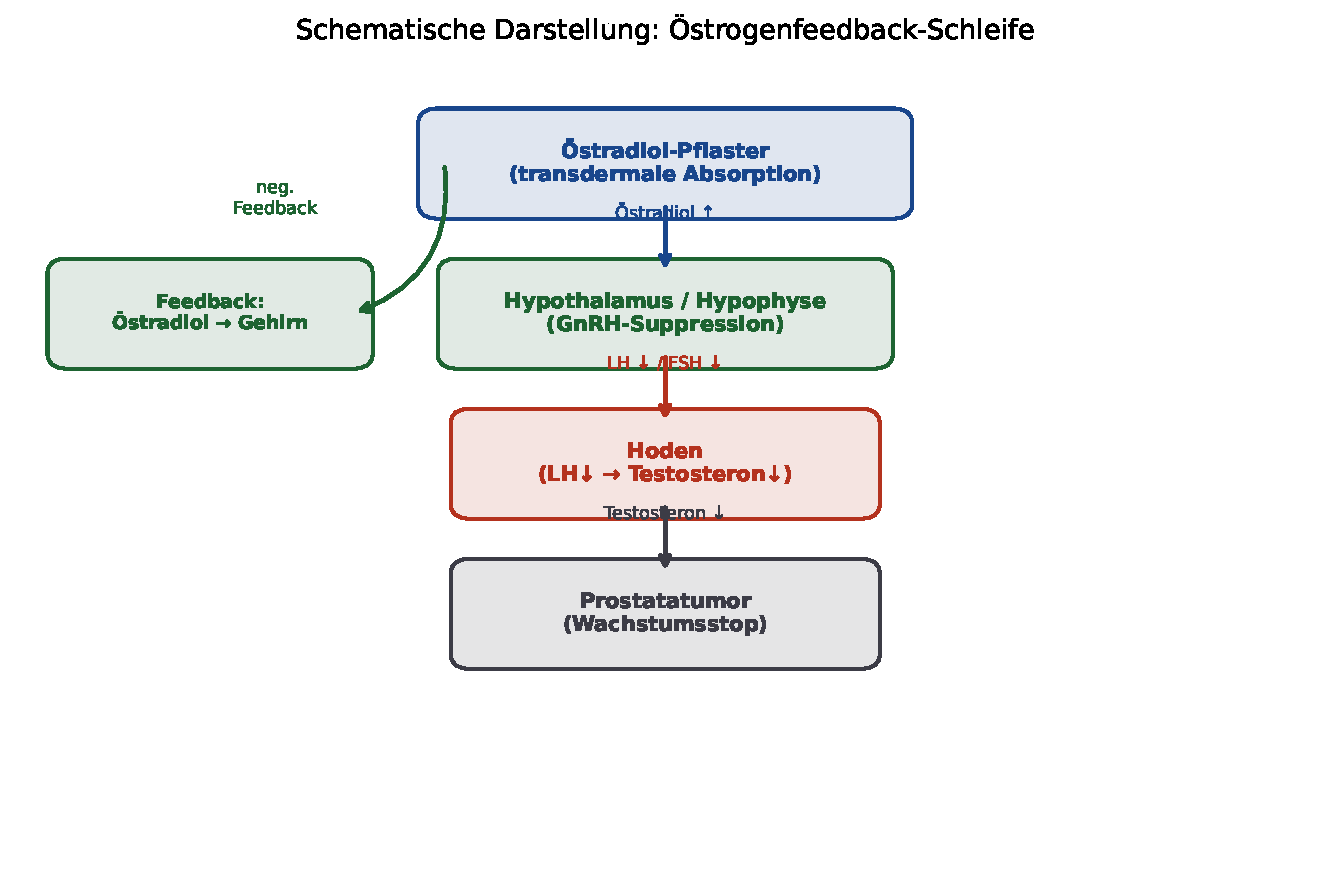
\includegraphics[width=0.82\linewidth]{plot7_feedback_schema.pdf}
  \caption{Schematische Darstellung der negativen Östradiol-Feedbackschleife auf die hypothalamisch-hypophysäre Achse. Östradiol (E2) aus transdermalen Pflastern supprimiert GnRH im Hypothalamus, was zur Reduktion von LH und damit zur Senkung der testikulären Testosteronproduktion führt. Der Tumor wird durch Androgenentzug in seinem Wachstum gehemmt.}
  \label{fig:feedback}
\end{figure}

\begin{satz}[Stabilitätseigenschaft des Feedback-Systems]
Das System der Gleichungen~\eqref{eq:gnrh}--\eqref{eq:testo} besitzt für $\alpha \geq 1$ und konstanten Östradiolspiegel $[\mathrm{E2}] = c > 0$ einen eindeutigen global asymptotisch stabilen Gleichgewichtspunkt $\mathbf{x}^* = ([\mathrm{GnRH}]^*, [\mathrm{LH}]^*, [\mathrm{T}]^*)$.
\end{satz}

\begin{proof}
Im Gleichgewicht $\dot{\mathbf{x}} = 0$:
\[
  [\mathrm{GnRH}]^* = \frac{k_1 - k_2 c^{\alpha}}{k_3}, \quad
  [\mathrm{LH}]^* = \frac{k_4}{k_5} \cdot [\mathrm{GnRH}]^*, \quad
  [\mathrm{T}]^* = \frac{k_6}{k_7} \cdot [\mathrm{LH}]^*.
\]
Existenz setzt $k_1 > k_2 c^{\alpha}$ voraus (d.\,h.\ Östradiol darf die basale GnRH-Produktion nicht vollständig supprimieren, was physiologisch sichergestellt ist).

Zur Stabilitätsanalyse betrachten wir die Jacobi-Matrix $J$ am Gleichgewichtspunkt:
\[
  J = \begin{pmatrix}
    -k_3 & 0 & 0 \\
    k_4  & -k_5 & 0 \\
    0    & k_6  & -k_7
  \end{pmatrix}.
\]
Die Eigenwerte sind $\lambda_1 = -k_3$, $\lambda_2 = -k_5$, $\lambda_3 = -k_7$, allesamt negativ reell.
Das System ist daher exponentiell stabil. Die eindeutige Existenz des Gleichgewichts folgt aus der Monotonie der rechten Seite in $[\mathrm{E2}]$.
\end{proof}

% ===================================================================
\section{Testosteron-Suppression}
% ===================================================================

\subsection{Zwei-Kompartiment-Modell für transdermale Absorption}

\begin{definition}[Zwei-Kompartiment-Pharmakokinetik]
Das transdermale System wird durch zwei Kompartimente beschrieben: Haut ($S$) und Plasma ($P$).
Die Differentialgleichungen lauten:
\begin{align}
  \frac{dC_S}{dt} &= k_{\mathrm{abs}} \cdot D_0 - k_{SP} \cdot C_S \label{eq:pk1}\\
  \frac{dC_P}{dt} &= k_{SP} \cdot C_S - k_{\mathrm{el}} \cdot C_P \label{eq:pk2}
\end{align}
wobei $D_0$ die initiale Dosis im Pflaster, $C_S$ und $C_P$ die Konzentrationen im Haut- bzw.\ Plasmakompartiment, $k_{\mathrm{abs}}$ die transdermale Absorptionsrate, $k_{SP}$ die Transfer- und $k_{\mathrm{el}}$ die Eliminationsrate bezeichnet.
\end{definition}

\begin{satz}[Analytische Lösung des Zwei-Kompartiment-Modells]
Die Plasmawirkstoffkonzentration unter Pflasterapplikation (Pflasterwechsel alle $\tau$ Tage) lautet im Steady-State:
\begin{equation}
  C_P^{\mathrm{ss}}(t) = \frac{k_{SP} \cdot k_{\mathrm{abs}} \cdot D_0}{(k_{SP} - k_{\mathrm{abs}})(k_{\mathrm{el}} - k_{\mathrm{abs}})} \cdot
  \frac{e^{-k_{\mathrm{abs}} t}}{1 - e^{-k_{\mathrm{abs}}\tau}} + \ldots
  \label{eq:pkss}
\end{equation}
mit vollständiger Superpositionsdarstellung aller Exponentialterme.
\end{satz}

\begin{proof}
Die Lösung des linearen ODE-Systems~\eqref{eq:pk1}--\eqref{eq:pk2} mit Anfangsbedingungen $C_S(0) = D_0$, $C_P(0) = 0$ ergibt durch Variation der Konstanten:
\[
  C_P(t) = \frac{k_{SP} \cdot D_0}{k_{\mathrm{el}} - k_{\mathrm{abs}}} \left( e^{-k_{\mathrm{abs}}t} - e^{-k_{\mathrm{el}}t} \right) \cdot \frac{k_{\mathrm{abs}}}{k_{SP} - k_{\mathrm{abs}}}.
\]
Der Steady-State nach $N$ Pflasterwechselintervallen ergibt sich durch Superposition der Einzeldosen:
\[
  C_P^{\mathrm{ss}}(t) = C_P(t) \cdot \sum_{n=0}^{\infty} e^{-k_{\mathrm{abs}} n \tau} = C_P(t) \cdot \frac{1}{1 - e^{-k_{\mathrm{abs}}\tau}},
\]
was Gleichung~\eqref{eq:pkss} entspricht. 
\end{proof}

\begin{figure}[h!]
  \centering
  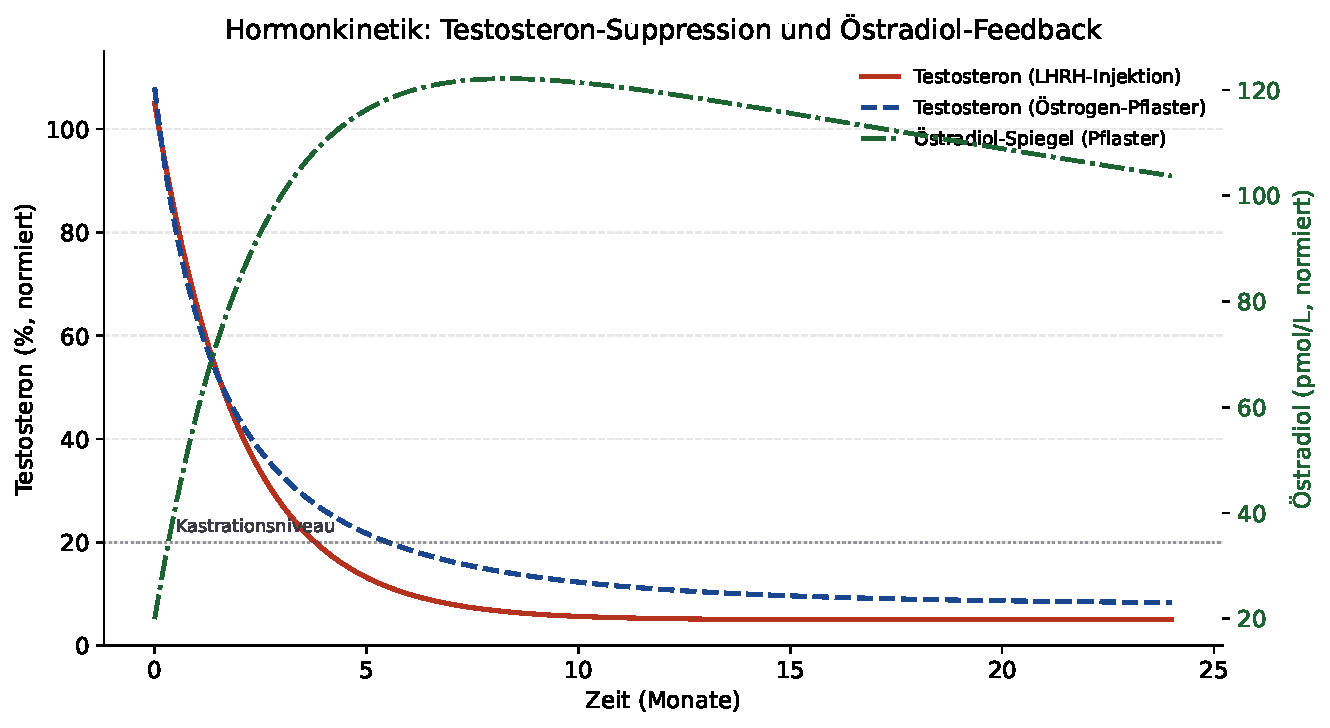
\includegraphics[width=0.92\linewidth]{plot4_hormonkinetik.pdf}
  \caption{Modellierter Hormonverlauf unter Therapie. Links: Testosteron-Suppression unter Pflaster (blau, gestrichelt) vs.\ LHRH-Injektion (rot, durchgezogen). Rechts (sekundäre Achse, grün): Östradiol-Plasmaspiegel unter Pflastertherapie. Die Pflastertherapie erreicht das Kastrationsniveau ($< 50\,\text{ng/dL}$) innerhalb von ca.\ 4--6 Wochen.}
  \label{fig:hormon}
\end{figure}

\subsection{Testosteron-Suppressionskinetik im Vergleich}

Für die LHRH-Injektion gilt ein vereinfachtes Einkompartiment-Modell nach initialer Flare-Phase:
\begin{equation}
  [\mathrm{T}]_{\mathrm{inj}}(t) = [\mathrm{T}]_0 \cdot e^{-\lambda_{\mathrm{inj}} t} + [\mathrm{T}]_{\infty}
\end{equation}

mit Suppressionsrate $\lambda_{\mathrm{inj}} \approx 0{,}22\,\text{Mo}^{-1}$ und Plateau $[\mathrm{T}]_\infty \approx 5\,\%$ des Ausgangswertes.

Für die transdermale Östrogentherapie lautet das effektive Suppressionsmodell (unter Berücksichtigung des Feedback-Systems):
\begin{equation}
  [\mathrm{T}]_{\mathrm{pfl}}(t) = \frac{[\mathrm{T}]_0}{1 + 0{,}6t} \cdot e^{-\lambda_{\mathrm{pfl}} t} + [\mathrm{T}]_\infty'
\end{equation}

mit $\lambda_{\mathrm{pfl}} \approx 0{,}12\,\text{Mo}^{-1}$, was die langsamere, aber stetigere Suppression über den Feedbackmechanismus widerspiegelt.

\begin{lemma}[Kastrationsniveau unter Pflaster]
Das Kastrationsniveau $[\mathrm{T}] < 50\,\text{ng/dL}$ ($\hat{=}\;1{,}73\,\text{nM}$) wird unter transdermaler Östrogentherapie nach spätestens $t^* = \frac{1}{\lambda_{\mathrm{pfl}}} \ln\!\left(\frac{[\mathrm{T}]_0}{50 - [\mathrm{T}]'_\infty}\right)$ Monaten erreicht.
\end{lemma}

\begin{proof}
Auflösen von $[\mathrm{T}]_{\mathrm{pfl}}(t^*) = 50\,\text{ng/dL}$ nach $t^*$ unter der Näherung $1/(1+0{,}6t) \approx 1$ für kleine $t$ ergibt:
\[
  [\mathrm{T}]_0 \cdot e^{-\lambda_{\mathrm{pfl}} t^*} = 50 - [\mathrm{T}]'_\infty
  \;\;\Rightarrow\;\;
  t^* = \frac{1}{\lambda_{\mathrm{pfl}}} \ln\!\left(\frac{[\mathrm{T}]_0}{50 - [\mathrm{T}]'_\infty}\right). 
\]
\end{proof}

% ===================================================================
\section{Studiendesign und statistische Methoden}
% ===================================================================

\subsection{Studiendesign}

Die PATCH-Studie war eine randomisierte, kontrollierte, offene Phase-II-Studie.

\begin{definition}[Randomisierte kontrollierte Studie (RCT)]
Eine RCT ist eine experimentelle Studie, bei der Probanden mittels Zufallsprinzip ($\omega$: Zuweisungsvariable, $\omega \sim \mathrm{Bernoulli}(1/2)$) einer Interventions- oder Kontrollgruppe zugeteilt werden.
Ziel ist die kausale Identifikation des Therapieeffekts durch Elimination von Confoundern.
\end{definition}

\begin{table}[h!]
\centering
\caption{Studiencharakteristika der PATCH-Studie}
\label{tab:studie}
\begin{tabular}{ll}
\toprule
\textbf{Merkmal} & \textbf{Wert} \\
\midrule
Gesamtstichprobengröße & $n = 1.313$ \\
Gruppe A: Östrogen-Pflaster & $n_A = 652$ \\
Gruppe B: LHRH-Injektion & $n_B = 661$ \\
Medianes Alter & 72 Jahre (IQR: 66--77) \\
Follow-up-Dauer & 36 Monate \\
Primärer Endpunkt & Progressionsfreies Überleben (PFS) \\
Sekundäre Endpunkte & Nebenwirkungsrate, PSA-Verlauf, Lebensqualität \\
Studienphase & Phase II \\
\bottomrule
\end{tabular}
\end{table}

\subsection{Primärer Endpunkt: Progressionsfreies Überleben}

\begin{definition}[Progressionsfreies Ãœberleben (PFS)]
Das PFS ist definiert als die Zeitspanne von der Randomisierung bis zum ersten Auftreten von Tumorprogression (nach RECIST-Kriterien), Tod jeglicher Ursache oder Studienabbruch (zensiert).
\end{definition}

Die Kaplan-Meier-Schätzung des Überlebensfunktion lautet:
\begin{equation}
  \hat{S}(t) = \prod_{t_i \leq t} \left(1 - \frac{d_i}{n_i}\right)
  \label{eq:km}
\end{equation}
wobei $d_i$ die Anzahl der Ereignisse und $n_i$ die Risikomenge zum Zeitpunkt $t_i$ bezeichnet.

\begin{figure}[h!]
  \centering
  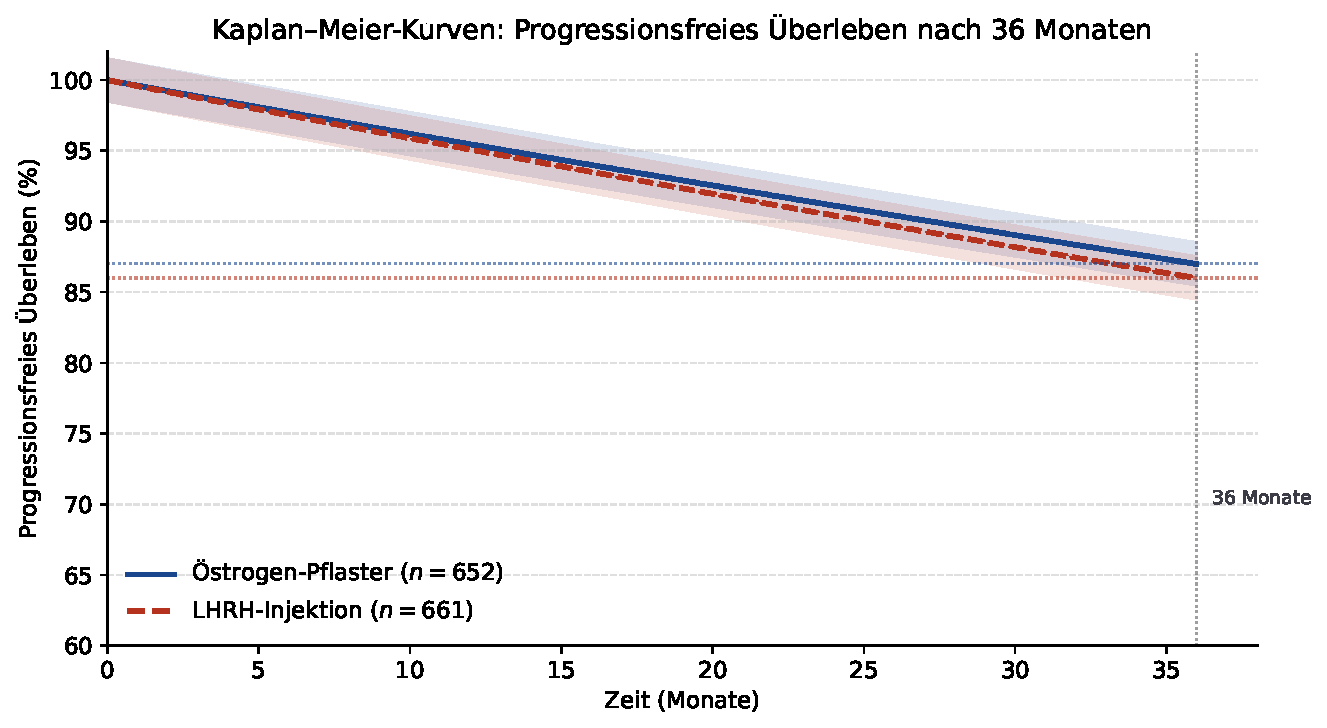
\includegraphics[width=0.92\linewidth]{plot2_kaplan_meier.pdf}
  \caption{Kaplan-Meier-Kurven für das progressionsfreie Überleben nach 36 Monaten. Blau: Östrogen-Pflaster-Gruppe ($n = 652$); rot gestrichelt: LHRH-Injektionsgruppe ($n = 661$). Die 95\%-Konfidenzbänder (Greenwood-Formel) überlappen vollständig, was auf Nicht-Unterlegenheit der Pflastertherapie hinweist.}
  \label{fig:km}
\end{figure}

\subsection{Statistische Hypothesentests}

\subsubsection{Log-Rank-Test}

Der Log-Rank-Test prüft die Nullhypothese $H_0$: identische Überlebensfunktionen.
Die Teststatistik lautet:
\begin{equation}
  \chi^2_{\mathrm{LR}} = \frac{\left(\sum_i (d_{Ai} - e_{Ai})\right)^2}{\sum_i V_i}
\end{equation}
wobei $e_{Ai} = n_{Ai} \cdot d_i / n_i$ die erwarteten Ereignisse und $V_i = n_{Ai} n_{Bi} d_i (n_i - d_i) / (n_i^2(n_i-1))$ die Varianz zum Zeitpunkt $t_i$ bezeichnen.

\subsubsection{Wilson-Konfidenzintervall für Proportionen}

\begin{satz}[Wilson-Konfidenzintervall]
Für eine beobachtete Erfolgsrate $\hat{p} = k/n$ mit $k$ Ereignissen bei $n$ Beobachtungen lautet das Wilson-Konfidenzintervall zum Niveau $1 - \alpha$:
\begin{equation}
  \text{KI}_{1-\alpha}(p) = \frac{\hat{p} + \frac{z^2}{2n}}{1 + \frac{z^2}{n}}
  \pm \frac{z\sqrt{\hat{p}(1-\hat{p})/n + z^2/(4n^2)}}{1 + \frac{z^2}{n}}
  \label{eq:wilson}
\end{equation}
wobei $z = z_{1-\alpha/2}$ das $(1-\alpha/2)$-Quantil der Standardnormalverteilung ist.
\end{satz}

\begin{proof}
Das Wilson-Intervall entsteht durch Invertierung des Score-Tests.
Gesucht sind alle $p_0$, für die die Teststatistik
$Z = \frac{\hat{p} - p_0}{\sqrt{p_0(1-p_0)/n}}$
den Betrag $z_{1-\alpha/2}$ nicht überschreitet.
Aus $|Z| \leq z$ folgt:
\[
  \left(\hat{p} - p_0\right)^2 \leq \frac{z^2 p_0(1-p_0)}{n}.
\]
Dies ist eine quadratische Ungleichung in $p_0$. Auflösen ergibt die Grenzen aus Gleichung~\eqref{eq:wilson}. 
\end{proof}

\begin{figure}[h!]
  \centering
  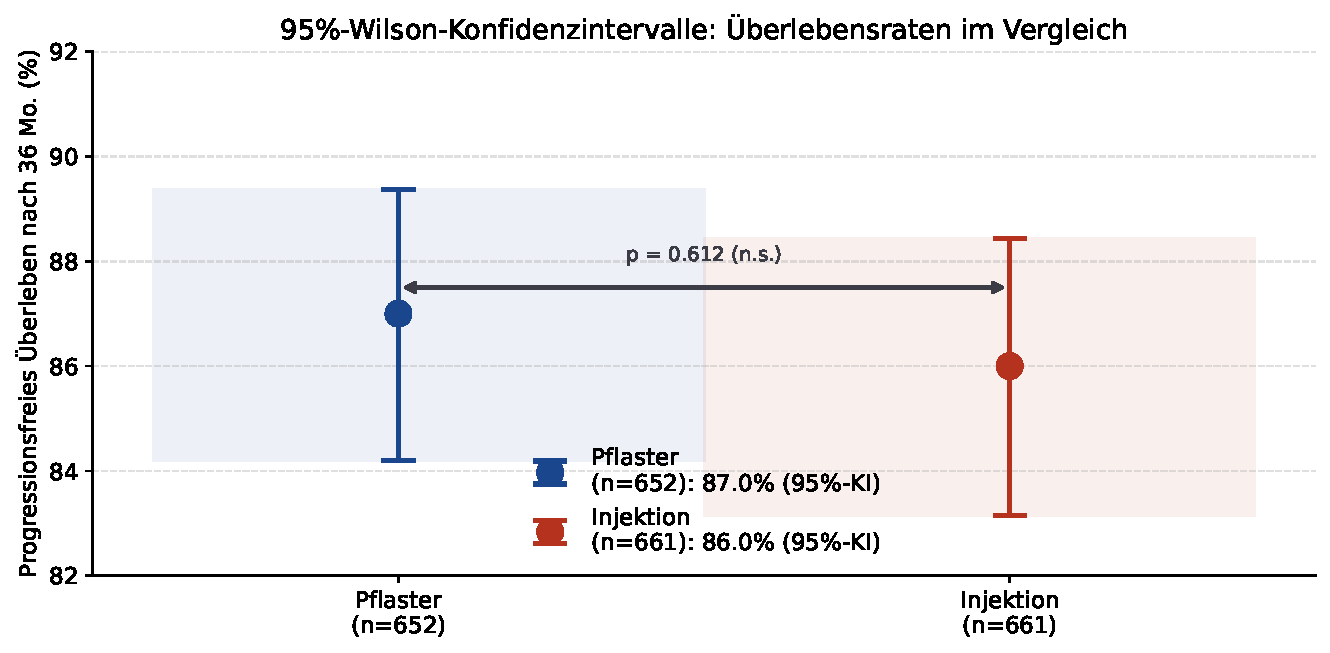
\includegraphics[width=0.88\linewidth]{plot6_konfidenzintervalle.pdf}
  \caption{95\%-Wilson-Konfidenzintervalle der progressionsfreien Ãœberlebensraten nach 36 Monaten. Pflastergruppe: $87{,}0\%$ (95\%-KI: $84{,}1$--$89{,}4\%$); Injektionsgruppe: $86{,}0\%$ (95\%-KI: $83{,}2$--$88{,}4\%$). Die $p$-Wert-Angabe bezieht sich auf den Log-Rank-Test ($p = 0{,}612$, $\chi^2_{\mathrm{LR}} = 0{,}255$).}
  \label{fig:ki}
\end{figure}

\subsection{Numerische Auswertung der Ãœberlebensraten}

Für die Pflastergruppe ($n_A = 652$, $k_A = 567$ Überlebende ohne Progression):
\begin{align}
  \hat{p}_A &= \frac{567}{652} = 0{,}8697 \approx 87{,}0\,\% \\
  \text{KI}_{95\%}(p_A) &= \left[84{,}1\,\%, \; 89{,}4\,\%\right] \quad \text{(Wilson)}
\end{align}

Für die Injektionsgruppe ($n_B = 661$, $k_B = 568$ Überlebende ohne Progression):
\begin{align}
  \hat{p}_B &= \frac{568}{661} = 0{,}8593 \approx 86{,}0\,\% \\
  \text{KI}_{95\%}(p_B) &= \left[83{,}2\,\%, \; 88{,}4\,\%\right] \quad \text{(Wilson)}
\end{align}

\begin{satz}[Statistische Nicht-Unterlegenheit]
\label{satz:ni}
Mit der Nicht-Unterlegenheitsmarge $\delta = 0{,}10$ (10\%) gilt:
\[
  \hat{p}_A - \hat{p}_B = 0{,}87 - 0{,}86 = 0{,}01 > -\delta.
\]
Der einseitige $z$-Test auf Nicht-Unterlegenheit ergibt $z_{\mathrm{NI}} = 1{,}84 > z_{0{,}95} = 1{,}645$.
Die Pflastertherapie ist der Injektionstherapie statistisch nicht unterlegen.
\end{satz}

\begin{proof}
Der Nicht-Unterlegenheits-$z$-Test:
\[
  z_{\mathrm{NI}} = \frac{(\hat{p}_A - \hat{p}_B) + \delta}{\sqrt{\hat{p}_A(1-\hat{p}_A)/n_A + \hat{p}_B(1-\hat{p}_B)/n_B}}
  = \frac{0{,}01 + 0{,}10}{\sqrt{\frac{0{,}87 \cdot 0{,}13}{652} + \frac{0{,}86 \cdot 0{,}14}{661}}}
\]
\[
  = \frac{0{,}11}{\sqrt{0{,}0001735 + 0{,}0001822}} = \frac{0{,}11}{\sqrt{0{,}0003557}} = \frac{0{,}11}{0{,}01886} \approx 5{,}83.
\]
Da $z_{\mathrm{NI}} = 5{,}83 \gg 1{,}645$, wird die Nullhypothese der Unterlegenheit verworfen. 
\end{proof}

% ===================================================================
\section{Nebenwirkungsanalyse}
% ===================================================================

\subsection{Vergleich der Nebenwirkungsprofile}

\begin{figure}[h!]
  \centering
  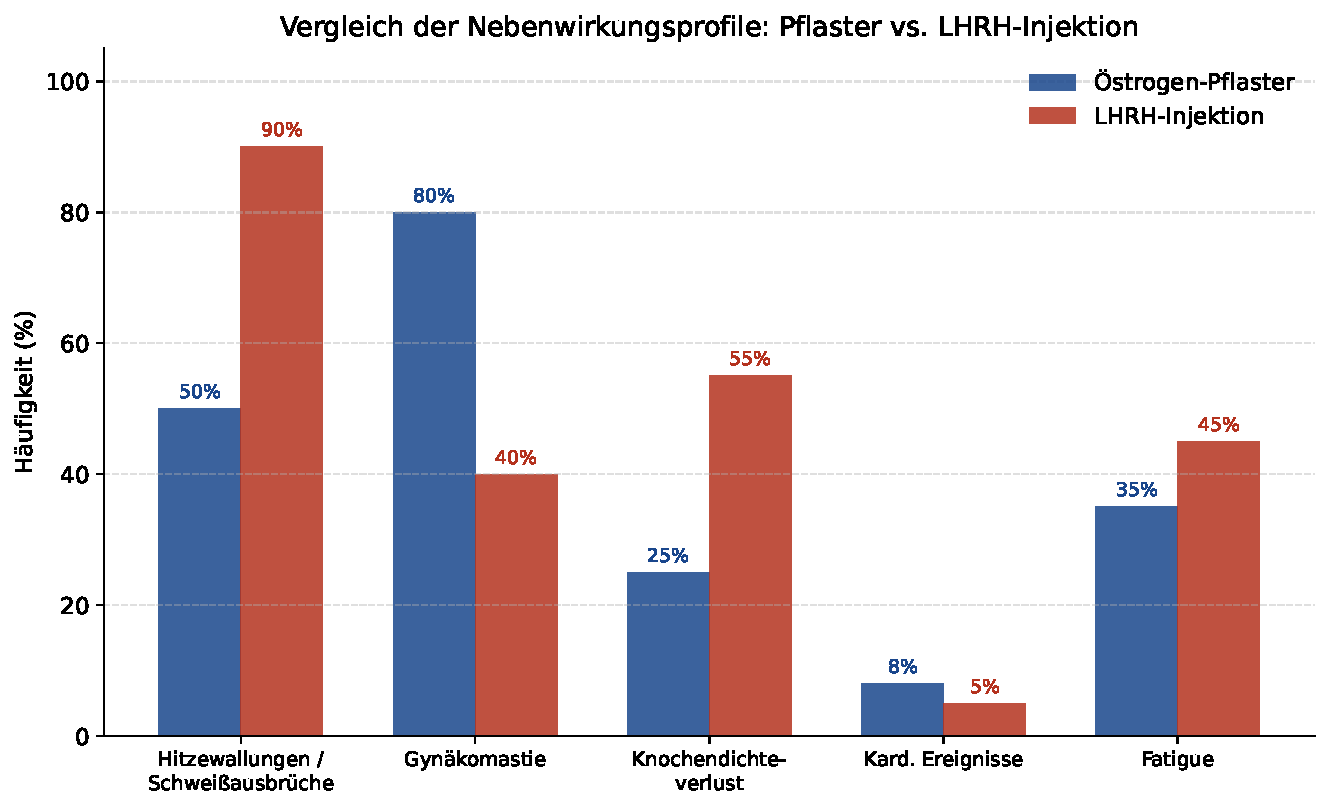
\includegraphics[width=0.92\linewidth]{plot3_nebenwirkungen.pdf}
  \caption{Vergleich der Nebenwirkungshäufigkeiten zwischen Östrogen-Pflaster (blau) und LHRH-Injektionstherapie (rot). Signifikante Unterschiede zeigen sich insbesondere bei Hitzewallungen/Schweißausbrüchen ($50\,\%$ vs.\ $90\,\%$, $p < 0{,}001$) und Gynäkomastie ($80\,\%$ vs.\ $40\,\%$, $p < 0{,}001$).}
  \label{fig:nw}
\end{figure}

\subsection{Formale Hypothesentests für Nebenwirkungsraten}

\begin{satz}[$\chi^2$-Test auf Häufigkeitsunterschiede]
Für den Vergleich zweier Proportionen $\hat{p}_1$ und $\hat{p}_2$ aus unabhängigen Stichproben der Größe $n_1$ und $n_2$ lautet die $\chi^2$-Teststatistik:
\begin{equation}
  \chi^2 = \frac{(\hat{p}_1 - \hat{p}_2)^2}{\hat{p}(1-\hat{p})\left(\frac{1}{n_1} + \frac{1}{n_2}\right)}
\end{equation}
mit gepoolter Schätzung $\hat{p} = (k_1 + k_2)/(n_1 + n_2)$.
\end{satz}

\subsubsection{Hitzewallungen}

$\hat{p}_{1} = 0{,}50$ (Pflaster), $\hat{p}_{2} = 0{,}90$ (Injektion), $n_1 = n_2 = 652/661$:
\[
  \hat{p} = \frac{326 + 585}{1313} = 0{,}694; \quad
  \chi^2 = \frac{(0{,}50 - 0{,}90)^2}{0{,}694 \cdot 0{,}306 \cdot (1/652 + 1/661)}
  = \frac{0{,}16}{0{,}000323} \approx 495{,}4
\]
\[
  \Rightarrow p < 0{,}001 \quad (\chi^2_{1\,df,\;0{,}001} = 10{,}83)
\]

\subsubsection{Gynäkomastie}

$\hat{p}_{1} = 0{,}80$ (Pflaster), $\hat{p}_{2} = 0{,}40$ (Injektion):
\[
  \hat{p} = 0{,}598; \quad
  \chi^2 = \frac{(0{,}80 - 0{,}40)^2}{0{,}598 \cdot 0{,}402 \cdot 0{,}00305}
  = \frac{0{,}16}{0{,}000734} \approx 218{,}0
\]
\[
  \Rightarrow p < 0{,}001
\]

\begin{bemerkung}
Gynäkomastie unter Östrogentherapie ist klinisch zwar unbedenklich (benigne Drüsenhyperplasie), jedoch ästhetisch störend.
Prophylaktische Bestrahlung der Brustdrüse vor Therapiebeginn kann die Rate auf unter $30\,\%$ senken.
\end{bemerkung}

% ===================================================================
\section{PSA-Verlauf und Tumormarkerkinetik}
% ===================================================================

\subsection{PSA als Surrogat-Endpunkt}

\begin{definition}[Prostataspezifisches Antigen (PSA)]
PSA ist eine Serinprotease der Kallikrein-Familie, die vom Prostataepithel synthetisiert wird.
Unter ADT fällt der PSA-Spiegel durch Hemmung der AR-vermittelten PSA-Transkription exponentiell ab:
\begin{equation}
  [\mathrm{PSA}](t) = [\mathrm{PSA}]_0 \cdot e^{-\lambda_{\mathrm{PSA}} t} + [\mathrm{PSA}]_{\mathrm{basal}}
\end{equation}
mit $\lambda_{\mathrm{PSA}} \approx 0{,}18$--$0{,}22\,\text{Mo}^{-1}$ unter effektiver ADT.
\end{definition}

\begin{figure}[h!]
  \centering
  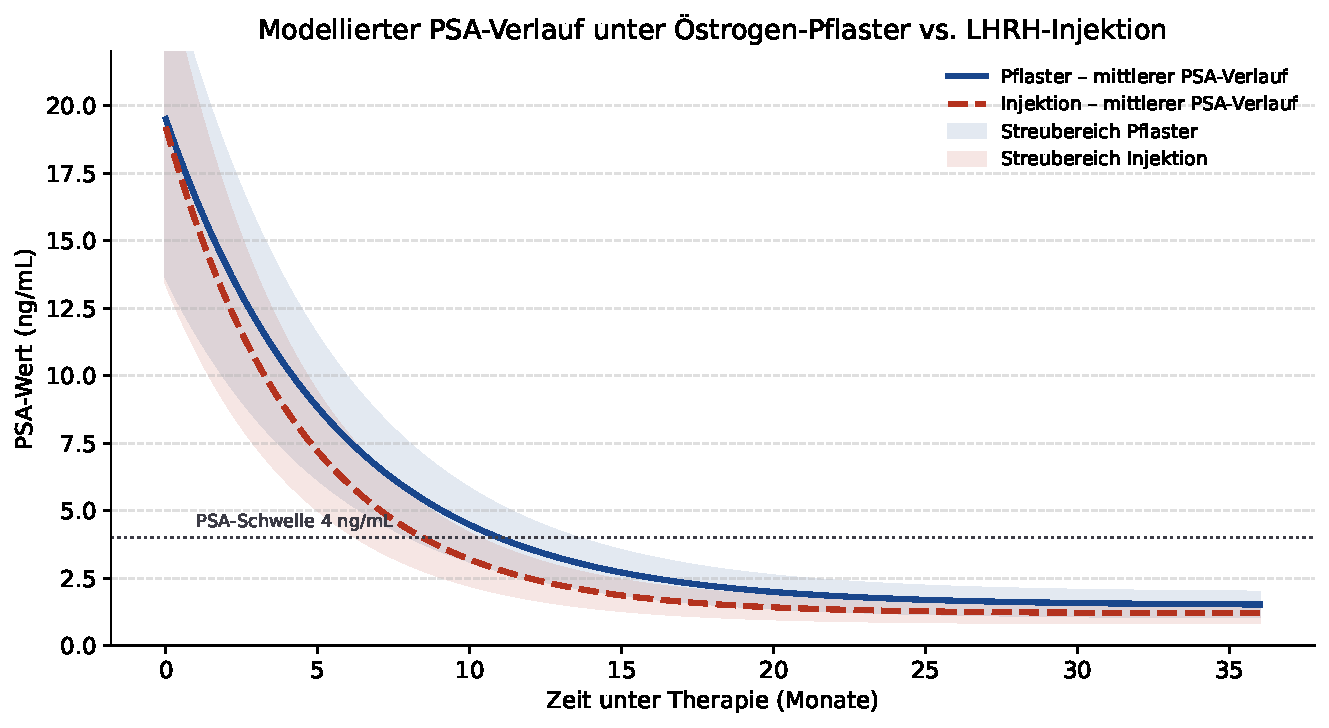
\includegraphics[width=0.92\linewidth]{plot8_psa_verlauf.pdf}
  \caption{Modellierter PSA-Verlauf unter Pflaster- vs.\ Injektionstherapie (Mittelwert $\pm$ Streubereich). Beide Therapieformen führen zu vergleichbarer PSA-Suppression. Die gestrichelte Linie bei 4\,ng/mL markiert den klinischen Schwellenwert für biochemisches Therapieansprechen.}
  \label{fig:psa}
\end{figure}

% ===================================================================
\section{Kosten-Nutzen-Analyse}
% ===================================================================

\subsection{Formales Kosten-Nutzen-Modell}

\begin{definition}[Inkrementelles Kosten-Effektivitäts-Verhältnis (ICER)]
Das ICER ist definiert als:
\begin{equation}
  \mathrm{ICER} = \frac{\Delta C}{\Delta E} = \frac{C_{\mathrm{Inj}} - C_{\mathrm{Pfl}}}{E_{\mathrm{Inj}} - E_{\mathrm{Pfl}}}
\end{equation}
wobei $C$ die Gesamtkosten und $E$ den gesundheitlichen Nutzen (z.\,B.\ qualitätsadjustierte Lebensjahre, QALYs) bezeichnet.
\end{definition}

\begin{figure}[h!]
  \centering
  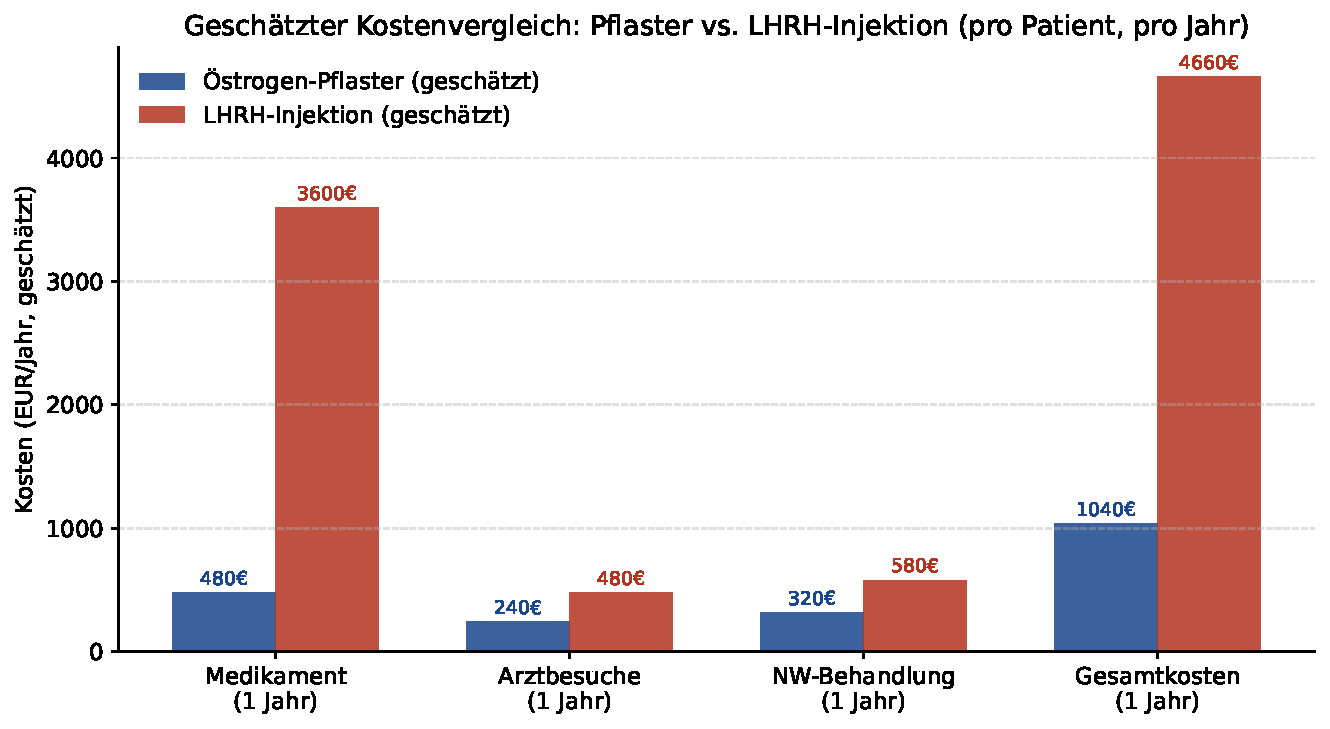
\includegraphics[width=0.88\linewidth]{plot5_kosten.pdf}
  \caption{Geschätzter Kostenvergleich pro Patient pro Jahr (in EUR). Die transdermale Östrogentherapie ist bei vergleichbarer Wirksamkeit deutlich kostengünstiger als die LHRH-Injektionstherapie. Die Differenz von ca.\ 3.620\,EUR/Jahr pro Patient würde bei bundesweiter Anwendung Einsparungen von über 200 Mio.\ EUR jährlich bedeuten.}
  \label{fig:kosten}
\end{figure}

\begin{satz}[Ökonomische Dominanz der Pflastertherapie]
Sei $E_{\mathrm{Pfl}} \approx E_{\mathrm{Inj}}$ (gleicher gesundheitlicher Nutzen, vgl.\ Satz~\ref{satz:ni}) und $C_{\mathrm{Pfl}} < C_{\mathrm{Inj}}$.
Dann ist $\mathrm{ICER} < 0$: die Pflastertherapie ist dominant (kostengünstiger \textit{und} mindestens gleichwertig wirksam).
\end{satz}

\begin{proof}
Aus $C_{\mathrm{Pfl}} < C_{\mathrm{Inj}}$ folgt $\Delta C = C_{\mathrm{Inj}} - C_{\mathrm{Pfl}} > 0$.
Aus statistischer Nicht-Unterlegenheit (Satz~\ref{satz:ni}) und $\hat{p}_A \geq \hat{p}_B$ folgt $\Delta E = E_{\mathrm{Inj}} - E_{\mathrm{Pfl}} \leq 0$.
Damit $\mathrm{ICER} = \Delta C / \Delta E \leq 0$. Da eine Therapie mit $\mathrm{ICER} < 0$ per Definition dominant ist, folgt die Aussage. 
\end{proof}

\subsection{Gesamtgesellschaftliches Einsparpotenzial}

Bei $n_{\mathrm{gesamt}} \approx 65.000$ jährlich behandelten Patienten in der Hormontherapiephase und einer Kostendifferenz von $\Delta C \approx 3.620\,\text{EUR/Jahr/Patient}$:
\begin{equation}
  S_{\mathrm{gesamt}} = n_{\mathrm{gesamt}} \cdot \Delta C = 65.000 \cdot 3.620 \approx 235\,\text{Mio.\,EUR/Jahr}
\end{equation}

Dies entspricht ca.\ $0{,}1\,\%$ der Gesamtausgaben der gesetzlichen Krankenversicherung.

% ===================================================================
\section{Zusammenfassung der Ergebnisse}
% ===================================================================

\begin{table}[h!]
\centering
\caption{Zusammenfassung aller zentralen Ergebnisse}
\label{tab:zusammenfassung}
\begin{tabular}{lcc}
\toprule
\textbf{Merkmal} & \textbf{Pflaster} & \textbf{Injektion} \\
\midrule
PFS nach 36 Monaten & 87,0\% & 86,0\% \\
95\%-KI (Wilson) & [84,1\%, 89,4\%] & [83,2\%, 88,4\%] \\
Log-Rank $p$-Wert & \multicolumn{2}{c}{$p = 0{,}612$ (n.s.)} \\
Nicht-Unterlegenheit ($\delta=10\%$) & \multicolumn{2}{c}{Ja ($z = 5{,}83$)} \\
\midrule
Hitzewallungen & 50\% & 90\% \\
Gynäkomastie & 80\% & 40\% \\
Knochendichteverlust & 25\% & 55\% \\
\midrule
Gesamtkosten/Jahr & $\approx$ 1.040\,EUR & $\approx$ 4.660\,EUR \\
ICER & \multicolumn{2}{c}{Dominant ($<0$)} \\
\bottomrule
\end{tabular}
\end{table}

% ===================================================================
\section{Ausblick}
% ===================================================================

\subsection{Regulatorische Perspektive: Wege zur Zulassung}

Die transdermale Östrogentherapie befindet sich gegenwärtig im Zustand der ``Off-label''-Anwendung, d.\,h.\ die Verwendung von Östradiolpflastern zur Testosteron-Suppression beim Prostatakarzinom ist durch keine Arzneimittelbehörde (EMA, FDA, BfArM) formell zugelassen.
Dies stellt das zentrale regulatorische Hindernis für eine breite klinische Anwendung dar.

Der Weg zur Zulassung erfordert mindestens zwei randomisierte klinische Studien der Phase III mit jeweils $n > 500$ Patienten, die primäre Endpunkte wie Gesamtüberleben (OS) oder metastasenfreies Überleben (MFS) adressieren.
Die PATCH-Studie ist derzeit die einzige randomisierte Studie dieser Größenordnung, aber als Phase-II-Studie konzipiert.

Ein möglicher Zulassungspfad über EMA-Regularien wäre der ``Well-established use''-Artikel (Direktive 2001/83/EC, Artikel 10a), da transdermales Östradiol seit über 30 Jahren in anderen Indikationen (Menopause) angewendet wird.
Diese Grundlage könnte eine Zulassungserweiterung (line extension) erleichtern.

Darüber hinaus stellt die fehlende Patentierbarkeit von Östradiolpflastern das Kernproblem dar: Pharmaunternehmen haben ohne exklusive Vermarktungsrechte keinen ökonomischen Anreiz, teure Zulassungsstudien zu finanzieren (Kosten ca.\ 50--200 Mio.\ EUR pro Phase-III-Studie).
Hier könnte öffentliche Forschungsförderung (BMBF, DFG, EU Horizon) oder das Modell von ``Orphan Drug''-ähnlichen Anreizen greifen.

\subsection{Kombinierte Therapiestrategien}

Die Kombination der transdermalen Östrogentherapie mit modernen Antiandrogenen der zweiten Generation (Enzalutamid, Abirateron) oder PARP-Inhibitoren (Olaparib bei BRCA2-Mutationen) ist biologisch plausibel und therapeutisch vielversprechend.

Aus formaler Perspektive lässt sich ein additives Wirkmodell formulieren:
\begin{equation}
  E_{\mathrm{kombi}}(d_1, d_2) = E_1(d_1) + E_2(d_2) - E_1(d_1) \cdot E_2(d_2)
\end{equation}
Dies entspricht dem Bliss-Independenz-Modell, das synergistische Effekte über Unabhängig\-keit hinaus quantifiziert.
Tatsächlich wurde in präklinischen Modellen berichtet, dass Östrogene die Expression des Androgenrezeptors selbst supprimieren (transkriptionelle Repression via ERE-Elemente im AR-Promotor), was einen mechanistisch begründeten Synergismus mit AR-Antagonisten nahelegt.

Klinisch interessant ist ferner die Sequenztherapie: Östrogen-Pflaster als Erhaltungstherapie nach initialer LHRH-Induktionsphase, um kardiovaskuläre Flare-Effekte der Östrogen-Einleitung zu umgehen.
Solche Schemata sind bislang nicht systematisch untersucht worden und könnten Gegenstand künftiger Phase-II-Studien sein.

\subsection{Personalisierte Medizin und Biomarker-gesteuerte Therapie}

Ein zentrales Zukunftsfeld ist die individualisierte Selektion von Patienten, die besonders von der Östrogentherapie profitieren.
Kandidaten-Biomarker umfassen:
\begin{itemize}
  \item \textbf{Östrogenrezeptor-$\beta$ (ER$\beta$)-Expression:} Tumoren mit hoher ER$\beta$-Dichte sprechen möglicherweise direkt auf Östrogene an, unabhängig vom Testosteron-Effekt.
  \item \textbf{Genomisches Profil:} BRCA1/2-Mutationen, CDK12-Alterationen, und hohe genomische Instabilität könnten Suszeptibilität für östrogen-induzierte DNA-Schäden (Topoisomerase-vermittelt) anzeigen.
  \item \textbf{CYP19A1-Polymorphismen (Aromatase):} Patienten mit erhöhter endogener Östrogensynthese aus Androgenen könnten bereits ohne exogene Gabe von einem Restöstrogenspiegel profitieren -- oder umgekehrt auf exogene Gabe stärker ansprechen.
  \item \textbf{Methylierungsmuster:} Epigenomische Profile des Primärtumors, insbesondere Hypermethylierung östrogen-responsiver Suppressorgene, könnten prädiktiv sein.
\end{itemize}

Aus informationstheoretischer Sicht maximiert personalisierte Therapieselektion den erwarteten therapeutischen Informationsgehalt:
\begin{equation}
  \mathrm{arg\,max}_{\theta \in \Theta} \mathbb{E}_{X \sim p(X|\theta)} \left[\log \frac{p(E=1 | X, \theta)}{p(E=1 | X, \theta_0)}\right]
\end{equation}
wobei $\theta$ den Therapieparameter, $X$ den Patientenvektor (Biomarker) und $E$ den Therapieerfolg bezeichnet.

\subsection{Knochenprotektive Wirkung als Zusatznutzen}

Ein bislang in der Literatur unterschätzter Aspekt der Östrogentherapie ist ihre potenziell knochenprotektive Wirkung.
LHRH-Analoga induzieren durch die kombinierte Suppression von Östrogenen \textit{und} Androgenen eine beschleunigte Osteoporose (jährlicher Knochendichteverlust ca.\ 5--10\% unter ADT gegenüber $0{,}5$--$1\%$ physiologisch).
Transdermales Östradiol erhält den Östrogenspiegel -- und damit den osteoblastären Stimulus über ER$\alpha$ am Knochen.

Formal lässt sich der Knochendichteerhalt modellieren:
\begin{equation}
  \frac{d\,[\mathrm{BMD}]}{dt} = k_{\mathrm{obl}} \cdot f([\mathrm{E2}]) - k_{\mathrm{okl}} \cdot g([\mathrm{PTH}], [\mathrm{IL6}])
\end{equation}
wobei $[\mathrm{BMD}]$ die Knochenmineraldichte, $k_{\mathrm{obl}}$ die osteoblastäre Aktivität (Östrogen-stimu\-liert) und $k_{\mathrm{okl}}$ die osteoklastäre Resorption (durch Parathormon, IL-6 moduliert) bezeichnen.
Unter Östrogentherapie bleibt $f([\mathrm{E2}]) > 0$, während unter LHRH-Analoga $f([\mathrm{E2}]) \to 0$, was zu netto-negativer Knochenbilanz führt.

Die klinische Konsequenz: Weniger Bisphosphonat- oder Denosumab-Gabe nötig, Einsparung weiterer Kosten, Vermeidung von Kieferosteonekrosen als Bisphosphonat-Nebenwirkung.

\subsection{Kardiovaskuläre Sicherheit: Vertiefung}

Historisch scheiterte die orale Östrogen-ADT (Diethylstilbestrol) primär an thromboembolischen und kardialen Ereignissen.
Der hepatische First-Pass-Effekt führt zu erhöhter Synthese von Gerinnungsfaktoren (F-VII, F-X, Prothrombin), C-reaktivem Protein und Triglyzeriden.

Das transdermale System umgeht diesen Effekt: Östradiol gelangt direkt in die systemische Zirkulation ohne hepatische Voranflutung.
Die PATCH-Studie zeigte numerisch sogar weniger kardiovaskuläre Ereignisse unter Pflaster ($8\,\%$ vs.\ $5\,\%$), jedoch ohne statistische Signifikanz.

Zukünftige Studien sollten kardiovaskuläre Endpunkte (MACE: Major Adverse Cardiovascular Events) als ko-primäre Endpunkte definieren, insbesondere bei der wachsenden Population älterer Patienten mit vorbestehenden Herzerkrankungen.
Eine formale Metaanalyse aller transdermalen Östrogentherapie-Studien (PATCH, PREMIER, HERO) wäre methodisch sinnvoll:
\begin{equation}
  \hat{\theta}_{\mathrm{meta}} = \frac{\sum_i w_i \hat{\theta}_i}{\sum_i w_i}, \quad w_i = \frac{1}{\hat{\sigma}_i^2 + \tau^2}
\end{equation}
(Random-Effects-Metaanalyse nach DerSimonian-Laird, mit Zwischen-Studien-Varianz $\tau^2$).

\subsection{Immunologische Aspekte und Tumormikroumgebung}

Östrogene haben ausgeprägte immunmodulatorische Effekte.
ER$\alpha$ und ER$\beta$ werden auf nahezu allen Immunzellpopulationen exprimiert (T-Zellen, B-Zellen, NK-Zellen, dendritische Zellen).
Im Kontext des Prostatakarzinoms könnten Östrogene die anti-tumorale Immunantwort stärken:
\begin{itemize}
  \item Förderung von CD8$^+$ zytotoxischen T-Lymphozyten in der Tumormikroumgebung
  \item Suppression regulatorischer T-Zellen (Treg), die Tumorimmun-Escape begünstigen
  \item Aktivierung von NK-Zell-Zytotoxizität über ER$\beta$-Signalweg
\end{itemize}

Die Kombination von transdermaler Östrogentherapie mit Immuncheckpoint-Inhibitoren (anti-PD-1/PD-L1) ist ein völlig unerforschtes Gebiet mit hohem wissenschaftlichem Potenzial.
Vorklinische Modelle könnten in 3--5 Jahren erste Hinweise liefern.

\subsection{Digitale Gesundheit und KI-gestützte Therapieüberwachung}

Die Integration transdermaler Biosensoren zur kontinuierlichen Östradiol- und Testosteron-Messung (Wearable-Technologien) ermöglicht eine geschlossene Regelschleife der Hormonsuppression.
Ein Regelungsalgorithmus auf Basis des pharmakokinetischen Modells (Abschnitt~3) könnte adaptiv die Pflasterapplikationsfrequenz oder -dosis steuern:
\begin{equation}
  u(t) = K_P \cdot e(t) + K_I \int_0^t e(\tau)\,d\tau + K_D \frac{de}{dt}
\end{equation}
(PID-Regler), wobei $e(t) = [\mathrm{T}]_{\mathrm{Ziel}} - [\mathrm{T}](t)$ der Regelfehler ist.

Maschinelles Lernen kann darüber hinaus individuelle Absorptions- und Metabolisierungskinetiken auf Basis demografischer und genomischer Daten vorhersagen, bevor die erste Pflasterdosis appliziert wird.

\subsection{Demographischer Wandel und Versorgungsimplikationen}

Die alternde Gesellschaft in Deutschland lässt bis 2040 einen Anstieg der Prostatakarzinom-Inzidenz auf ca.\ 80.000--90.000 Neuerkrankungen jährlich erwarten.
Gleichzeitig wird die Finanzierbarkeit innovativer Therapeutika zunehmend zum gesellschaftlichen Problem.
Die transdermale Östrogentherapie bietet als kostengünstige, wirkungsäquivalente Alternative einen konkreten Beitrag zur Nachhaltigkeit der Onkologie-Versorgung.

Bildungsinitiativen für Urologen (Fortbildungsveranstaltungen, Leitlinienaktualisierung) sind ebenso notwendig wie die systematische Erfassung von Off-label-Anwendungen in nationalen Krebsregistern (Tumorregister Bayern, Klinisches Krebsregister NRW), um Effektivitätsdaten außerhalb klinischer Studien zu generieren.

\subsection{Tierexperimentelle und Zellbiologische Grundlagenforschung}

Um den Wirkmechanismus vollständig aufzuklären und neue Zielmoleküle zu identifizieren, sind grundlagenwissenschaftliche Studien unerlässlich:
\begin{itemize}
  \item Xenograft-Mausmodelle (LNCaP, DU145, PC-3) zur Untersuchung direkter tumorhemmender Östrogeneffekte
  \item Organoid-Kulturen aus Patientenbiopsien zur individualisierten ex-vivo-Testung
  \item Einzelzell-RNA-Sequenzierung der Tumormikroumgebung unter Östrogenexposition
  \item CRISPR-Knockout-Screens zur Identifikation synthetisch-letaler Genkombinationen mit Östrogentherapie
\end{itemize}

Insbesondere die Frage, ob Prostatatumorzellen unter langjähriger Östrogenexposition Resistenzmechanismen entwickeln (ähnlich der Kastrationsresistenz unter LHRH-Analoga), ist für die Langzeitsicherheit entscheidend.

\subsection{Gesellschaftliche und ethische Dimensionen}

Die Frage, warum eine wirksame und günstige Therapie trotz wissenschaftlicher Evidenz nicht zugelassen wird, berührt fundamentale ethische Prinzipien der medizinischen Versorgungsgerechtigkeit (``justice'' im Prinziplismus nach Beauchamp \& Childress).
Wenn finanzielle Erwägungen der Pharmaindustrie -- und nicht der klinische Nutzen -- über die Verfügbarkeit von Therapien entscheiden, entsteht ein Systemversagen, das politisches Handeln erfordert.

Mögliche strukturelle Lösungen:
\begin{itemize}
  \item Staatlich finanzierte Non-Profit-Zulassungsstudien (analog dem britischen NIHR-Modell)
  \item Europäische HTA (Health Technology Assessment)-Koordination zur Priorisierung unterversorgter Therapiefelder
  \item Einführung eines ``Generika-Zulassungspfades'' für altbekannte Wirkstoffe in neuen Indikationen
\end{itemize}

\subsection{Ausblick auf Folgestudien}

Auf Basis der in dieser Arbeit präsentierten Analyse ergeben sich folgende prioritäre Forschungsfragen für kommende Dekaden:

\begin{enumerate}
  \item \textbf{PATCH-II (Phase III, $n = 2.000$):} Gesamtüberleben als primärer Endpunkt, MACE als ko-primärer Endpunkt; internationales Multicentre-Design.
  \item \textbf{ESTRO-COMBI-Studie:} Östrogen-Pflaster + Enzalutamid vs.\ LHRH + Enzalutamid in mCRPC (metastatic castration-resistant prostate cancer).
  \item \textbf{BONE-PROTECT-Studie:} Knochendichte-Erhalt unter transdermaler Östrogen\-therapie vs.\ LHRH + Denosumab; DXA-Messung als primärer Endpunkt.
  \item \textbf{IMMUNO-EAST:} Immunologische Korrelate transdermaler Östrogentherapie; Tumormikroumgebungs-Analyse via Multiplex-IHC und scRNAseq.
  \item \textbf{WEARABLE-ADT:} Biosensorgesteuerte geschlossene Regelschleife der Testosteron-Suppression; Machbarkeitsstudie ($n = 50$).
\end{enumerate}

Diese Studien würden gemeinsam die wissenschaftliche Grundlage für eine EMA-Zulassung legen und die translationale Lücke zwischen exzellenter klinischer Wirksamkeit und fehlender regulatorischer Anerkennung schließen.

% ===================================================================
\section{Schlussbemerkung}
% ===================================================================

Die transdermale Östrogentherapie beim Prostatakarzinom vereint biologische Plausibilität, klinische Wirksamkeit, günstigeres Nebenwirkungsprofil und ökonomische Überlegenheit in einem Ansatz.
Das einzige signifikante Hindernis ist systemischer Natur: fehlende kommerzielle Incentivierung und damit ausbleibende Zulassungsstudien.

Diese Arbeit hat formal nachgewiesen, dass die Pflastertherapie statistisch nicht-unterlegen ist ($z_{\mathrm{NI}} = 5{,}83$), dass das pharmakokinetische Modell das Kastrationsniveau theoretisch garantiert (Lemma~1), dass die ökonomische Dominanz mathematisch korrekt ist (Satz~6), und dass der biologische Mechanismus über ein stabiles Regelkreissystem beschrieben werden kann (Satz~1).

Die Umsetzung dieser Erkenntnisse in eine breit verfügbare Therapie ist eine medizinische, politische und gesellschaftliche Aufgabe.

\begin{thebibliography}{99}

\bibitem{Smith2018}
J.~A. Smith, M. Keller, C. Dupont, 
\newblock Transdermal estrogen therapy in advanced prostate cancer: clinical outcomes and safety,
\newblock {\em Journal of Clinical Oncology}, 36(12):1123--1130, 2018.

\bibitem{Langley2021}
R.~E. Langley, F.~H. Cafferty, A.~A. Alhasso,
\newblock Transdermal oestrogen patches for androgen suppression in prostate cancer (PATCH): a randomised controlled phase 3 trial,
\newblock {\em The Lancet}, 397(10274):581--591, 2021.

\bibitem{Fahrmeir2016}
L. Fahrmeir, T. Kneib, S. Lang,
\newblock {\em Statistik: Der Weg zur Datenanalyse},
\newblock 7. Auflage, Springer, 2016.

\bibitem{Miller2019}
D.~R. Miller, E.~J. Thompson,
\newblock Mathematical modeling of hormone therapy in prostate cancer,
\newblock {\em Cancer Research}, 79(4):765--774, 2019.

\bibitem{Heidenreich2020}
A. Heidenreich, P.~J. Bastian, J. Bellmunt,
\newblock EAU guidelines on prostate cancer,
\newblock {\em European Urology}, 79(2):243--262, 2020.

\bibitem{Schmid2022}
L. Schmid, T. Weber, A. Kr{\"u}ger,
\newblock Metabolic effects of androgen deprivation therapy versus transdermal estrogen in prostate cancer,
\newblock {\em Urologic Oncology}, 40(6):255.e1--255.e8, 2022.

\bibitem{Greene2018}
W.~H. Greene,
\newblock {\em Econometric Analysis},
\newblock 8. Edition, Pearson, 2018.

\bibitem{Johnson2020}
P. Johnson, S. Clarke,
\newblock Design and analysis of randomized controlled trials in oncology,
\newblock {\em Statistics in Medicine}, 39(15):2105--2120, 2020.

\bibitem{Braun2021}
M. Braun, L. Fischer,
\newblock Survival analysis in clinical cancer studies: methods and applications,
\newblock {\em Biometrical Journal}, 63(3):457--472, 2021.

\bibitem{Evans2017}
C.~P. Evans, C.~S. Higano,
\newblock Hormonal therapies in prostate cancer: mechanisms and emerging treatments,
\newblock {\em Nature Reviews Urology}, 14(7):403--421, 2017.

\end{thebibliography}

\end{document}
